\documentclass[unicode,11pt,a4paper,oneside,numbers=endperiod,openany]{scrartcl}

\usepackage{ifthen}
\usepackage[utf8]{inputenc}
\usepackage{graphics}
\usepackage{graphicx}
\usepackage{hyperref}

\pagestyle{plain}
\voffset -5mm
\oddsidemargin  0mm
\evensidemargin -11mm
\marginparwidth 2cm
\marginparsep 0pt
\topmargin 0mm
\headheight 0pt
\headsep 0pt
\topskip 0pt        
\textheight 255mm
\textwidth 165mm

\newcommand{\duedate} {}
\newcommand{\setduedate}[1]{%
\renewcommand\duedate {See iCorsi for due date}}
\newcommand\isassignment {false}
\newcommand{\setassignment}{\renewcommand\isassignment {true}}
\newcommand{\ifassignment}[1]{\ifthenelse{\boolean{\isassignment}}{#1}{}}
\newcommand{\ifnotassignment}[1]{\ifthenelse{\boolean{\isassignment}}{}{#1}}

\newcommand{\assignmentpolicy}{
\begin{table}[h]
\begin{center}
\scalebox{0.8} {%
\begin{tabular}{|p{0.02cm}p{16cm}|}
\hline
&\\
\multicolumn{2}{|c|}{\Large\textbf{HPC Lab ---  Submission Instructions}}\\
\multicolumn{2}{|c|}{\large\textbf{(Please, notice that following instructions are mandatory: }}\\
\multicolumn{2}{|c|}{\large\textbf{submissions that don't comply with, won't be considered)}}\\
&\\
\textbullet & Assignments must be submitted to \href{https://www.icorsi.ch}{iCorsi} (i.e. in electronic format).\\
\textbullet & Provide source files (e.g. C/C++ files, Matlab). 
If you are using libraries, please add them in the file. Sources must be organized in directories called:\\
\multicolumn{2}{|c|}{\textit{Project\_number\_lastname\_firstname}}\\
& and  the  file must be called:\\
\multicolumn{2}{|c|}{\textit{project\_number\_lastname\_firstname.zip}}\\
\multicolumn{2}{|c|}{\textit{project\_number\_lastname\_firstname.pdf}}\\
\textbullet &  The TAs will grade your project by reviewing your project write-up, and looking at the implementation 
                 you attempted, and benchmarking your code's performance.\\

\textbullet & You are allowed to discuss all questions with anyone you like; however: (i) your submission must list anyone you discussed problems with and (ii) you must write up your submission independently.\\
\hline
\end{tabular}
}
\end{center}
\end{table}
}
\newcommand{\punkte}[1]{\hspace{1ex}\emph{\mdseries\hfill(#1~\ifcase#1{Points}\or{Points}\else{Points}\fi)}}


\newcommand\serieheader[6]{
\thispagestyle{empty}%
\begin{flushleft}

\includegraphics[width=0.4\textwidth]{usi_inf.png}
\end{flushleft}
  \noindent%
  {\large\ignorespaces{\textbf{#1}}\hspace{\fill}\ignorespaces{ \textbf{#2}}}\\ \\%
  {\large\ignorespaces #3 \hspace{\fill}\ignorespaces #4}\\
  \noindent%
  \bigskip
  \hrule\par\bigskip\noindent%
  \bigskip {\ignorespaces {\Large{\textbf{#5}}}
  \hspace{\fill}\ignorespaces \large \ifthenelse{\boolean{\isassignment}}{\duedate}{#6}}
  \hrule\par\bigskip\noindent%  \linebreak
 }

\makeatletter
\def\enumerateMod{\ifnum \@enumdepth >3 \@toodeep\else
      \advance\@enumdepth \@ne
      \edef\@enumctr{enum\romannumeral\the\@enumdepth}\list
      {\csname label\@enumctr\endcsname}{\usecounter
        {\@enumctr}%%%? the following differs from "enumerate"
	\topsep0pt%
	\partopsep0pt%
	\itemsep0pt%
	\def\makelabel##1{\hss\llap{##1}}}\fi}
\let\endenumerateMod =\endlist
\makeatother




\usepackage{textcomp}





\usepackage{listings}
\usepackage{hyperref}
\usepackage{subcaption}
\usepackage{multirow}
\usepackage{float}
\usepackage{xcolor}
\usepackage{csvsimple}

\usepackage[T1]{fontenc}
\usepackage{inconsolata}

\lstdefinestyle{hpcblock}{
    basicstyle=\ttfamily\footnotesize,
    backgroundcolor=\color{gray!10},
    frame=single,
    rulecolor=\color{gray!60},
    xleftmargin=1.5em,
    xrightmargin=1.5em,
    aboveskip=1em,
    belowskip=1em,
    showstringspaces=false,
    columns=fullflexible,
    keepspaces=true,
    breaklines=true,
    postbreak=\mbox{\textcolor{gray}{$\hookrightarrow$}\space}
}
\lstset{style=hpcblock}

\begin{document}

\setassignment

\serieheader{High-Performance Computing Lab}{Institute of Computing}{Student: Paolo Deidda}{Discussed with: --}{Solution for Project 2}{}
\newline

\assignmentpolicy
This project will introduce you to parallel programming using OpenMP. 

\tableofcontents
\newpage




\section{Parallel reduction operations using OpenMP \punkte{20}}
\subsection{Dot product}

\subsubsection{Implementation}
I compiled \texttt{Skeleton\_codes/dotProduct/dotProduct.cpp} with \texttt{g++ -fopenmp}. The Makefile exposes the vector size through the variable \texttt{N}, injected at compile time (``\texttt{-DN=\$(N)}''). The batch script \texttt{run\_jobs.sh} rebuilds the binary for each $N \in \{10^5,10^6,10^7,10^8\}$ and runs both OpenMP variants.

\lstinputlisting[
    caption={Reduction-based OpenMP dot product},
    captionpos=b,
    label={lst:dotprod_reduction},
    language=C++,
    numbers=left,
    linerange={57-67},
    firstnumber=57
]{../Skeleton_codes/dotProduct/dotProduct.cpp}

Listing~\ref{lst:dotprod_reduction} lets OpenMP handle partial sums via the \texttt{reduction} clause, avoiding explicit synchronisation. The alternative keeps thread-local buffers and merges them inside a \texttt{critical} region, shown in Listing~\ref{lst:dotprod_critical}.

\lstinputlisting[
    caption={Critical-based OpenMP dot product},
    captionpos=b,
    label={lst:dotprod_critical},
    language=C++,
    numbers=left,
    linerange={69-84},
    firstnumber=69
]{../Skeleton_codes/dotProduct/dotProduct.cpp}


\subsubsection{Testing}
For each size the script sweeps \texttt{OMP\_NUM\_THREADS} in $\{1,2,4,8,16,20\}$, exporting the value before invoking the executable. Each run stores its stdout to \texttt{logs/dotprod\_N\ldots\_T\ldots.log}; a Python helper converts the logs into the plots below and verifies that the reduction and critical versions match the serial dot product within a relative tolerance of $10^{-6}$.

\subsubsection{Discussion}
Figures~\ref{fig:dotprod_n1e5}--\ref{fig:dotprod_n1e8} show that even the smallest test ($N = 10^5$) benefits from parallelism: two threads reduce the runtime from $11.7\,\mathrm{ms}$ to $6.2\,\mathrm{ms}$ and eight threads reach $2.4\,\mathrm{ms}$. The efficiency plot in Figure~\ref{fig:dotprod_eff} highlights how OpenMP overhead grows with the thread count: efficiency is defined as $E = T_1 /(p \cdot T_p)$, so every time the speedup grows sub-linearly the per-core return decreases (e.g.\ speedup $\approx 2$ on two threads gives $E \approx 1$, speedup $\approx 4.9$ on eight threads gives $E \approx 0.6$). Beyond eight threads the serial portion and the \texttt{critical} synchronisation dominate, so efficiencies fall below $0.3$, even though the absolute runtime still drops (e.g.\ $T_{16} = 0.54\,\mathrm{s}$ for $N = 10^7$). The reduction variant consistently retains $5{-}10\%$ higher efficiency because it avoids serialised updates. Overall, multi-threading is worth, provided that the thread count remains modest (up to eight) to keep overhead under control for the smaller vectors; for $N \ge 10^7$ the reduction version scales well up to sixteen threads.

\begin{figure}[H]
    \centering
    \begin{subfigure}{0.45\textwidth}
        \centering
        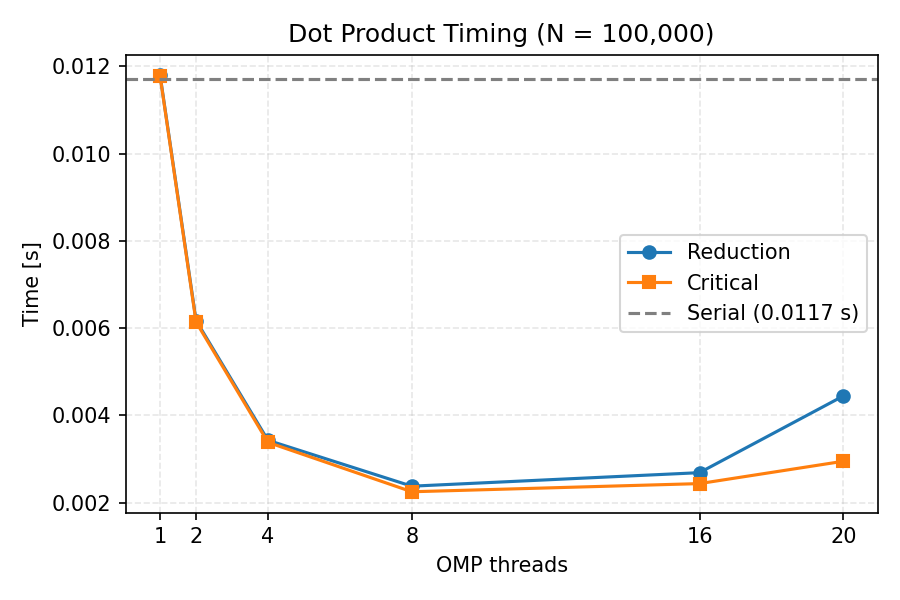
\includegraphics[width=\linewidth]{../Skeleton_codes/dotProduct/plots/dotprod_N100000.png}
        \caption{$N = 10^5$}
        \label{fig:dotprod_n1e5}
    \end{subfigure}
    \hfill
    \begin{subfigure}{0.45\textwidth}
        \centering
        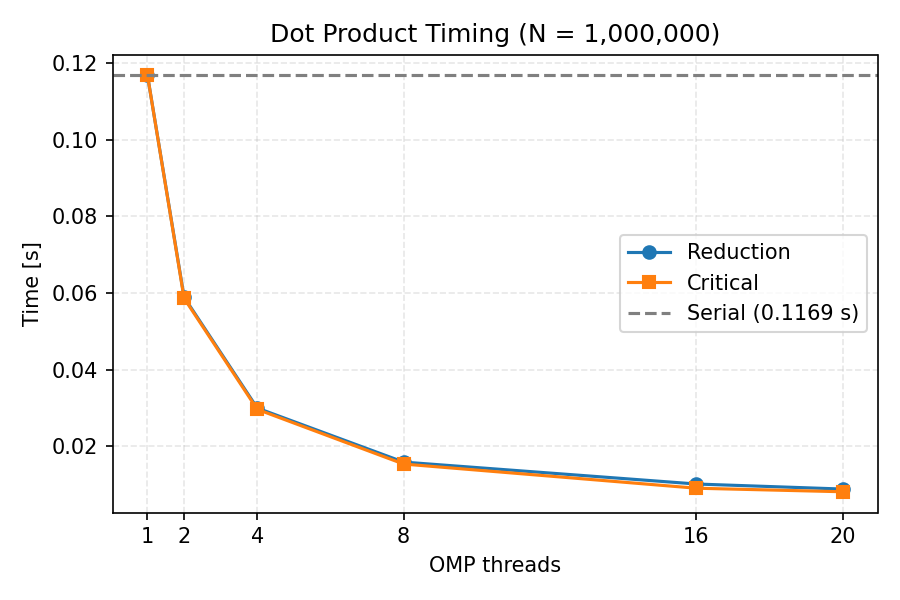
\includegraphics[width=\linewidth]{../Skeleton_codes/dotProduct/plots/dotprod_N1000000.png}
        \caption{$N = 10^6$}
        \label{fig:dotprod_n1e6}
    \end{subfigure}

    \vspace{1em}

    \begin{subfigure}{0.45\textwidth}
        \centering
        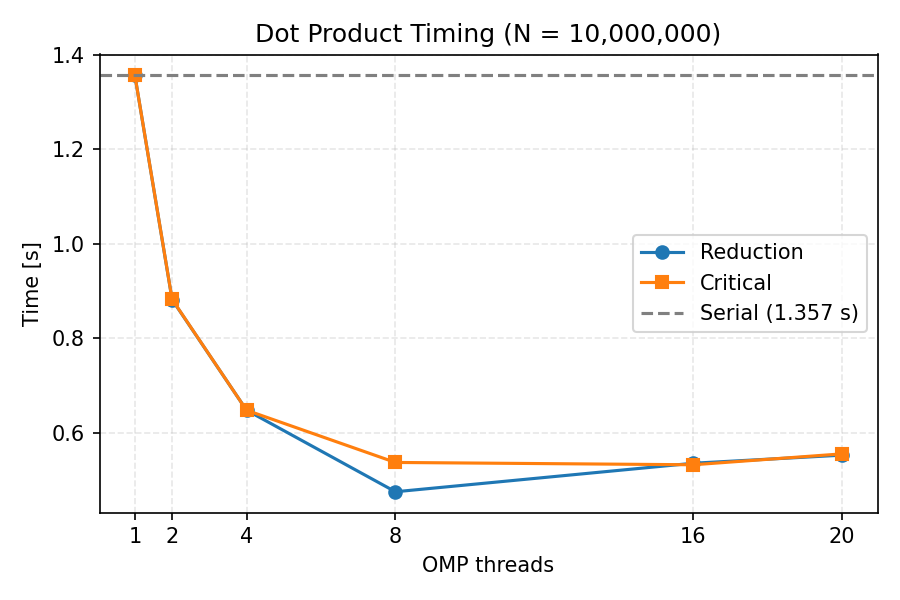
\includegraphics[width=\linewidth]{../Skeleton_codes/dotProduct/plots/dotprod_N10000000.png}
        \caption{$N = 10^7$}
        \label{fig:dotprod_n1e7}
    \end{subfigure}
    \hfill
    \begin{subfigure}{0.45\textwidth}
        \centering
        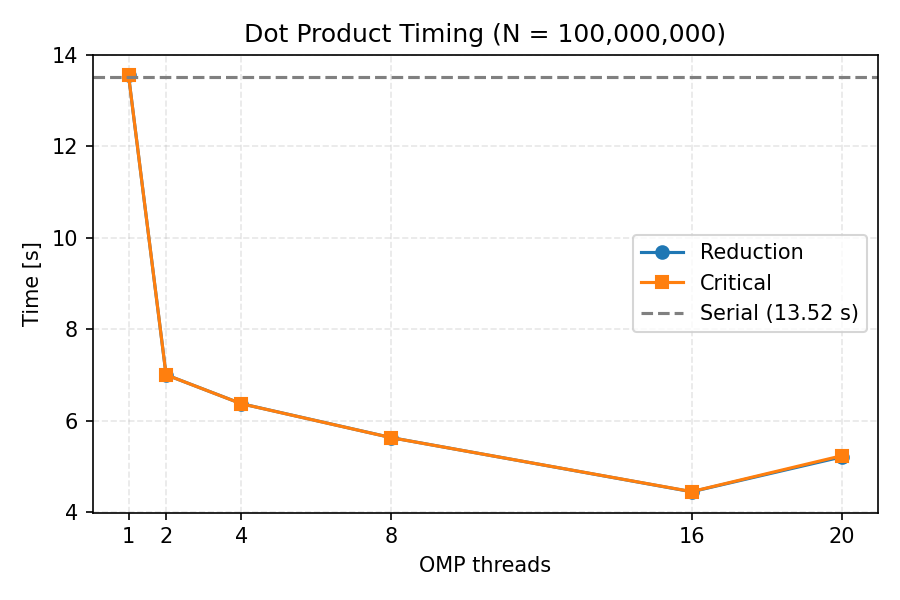
\includegraphics[width=\linewidth]{../Skeleton_codes/dotProduct/plots/dotprod_N100000000.png}
        \caption{$N = 10^8$}
        \label{fig:dotprod_n1e8}
    \end{subfigure}
    \caption{Execution time vs. threads for different vector sizes.}
\end{figure}

\begin{figure}[H]
    \centering
    \IfFileExists{../Skeleton_codes/dotProduct/plots/dotprod_efficiency.png}{
        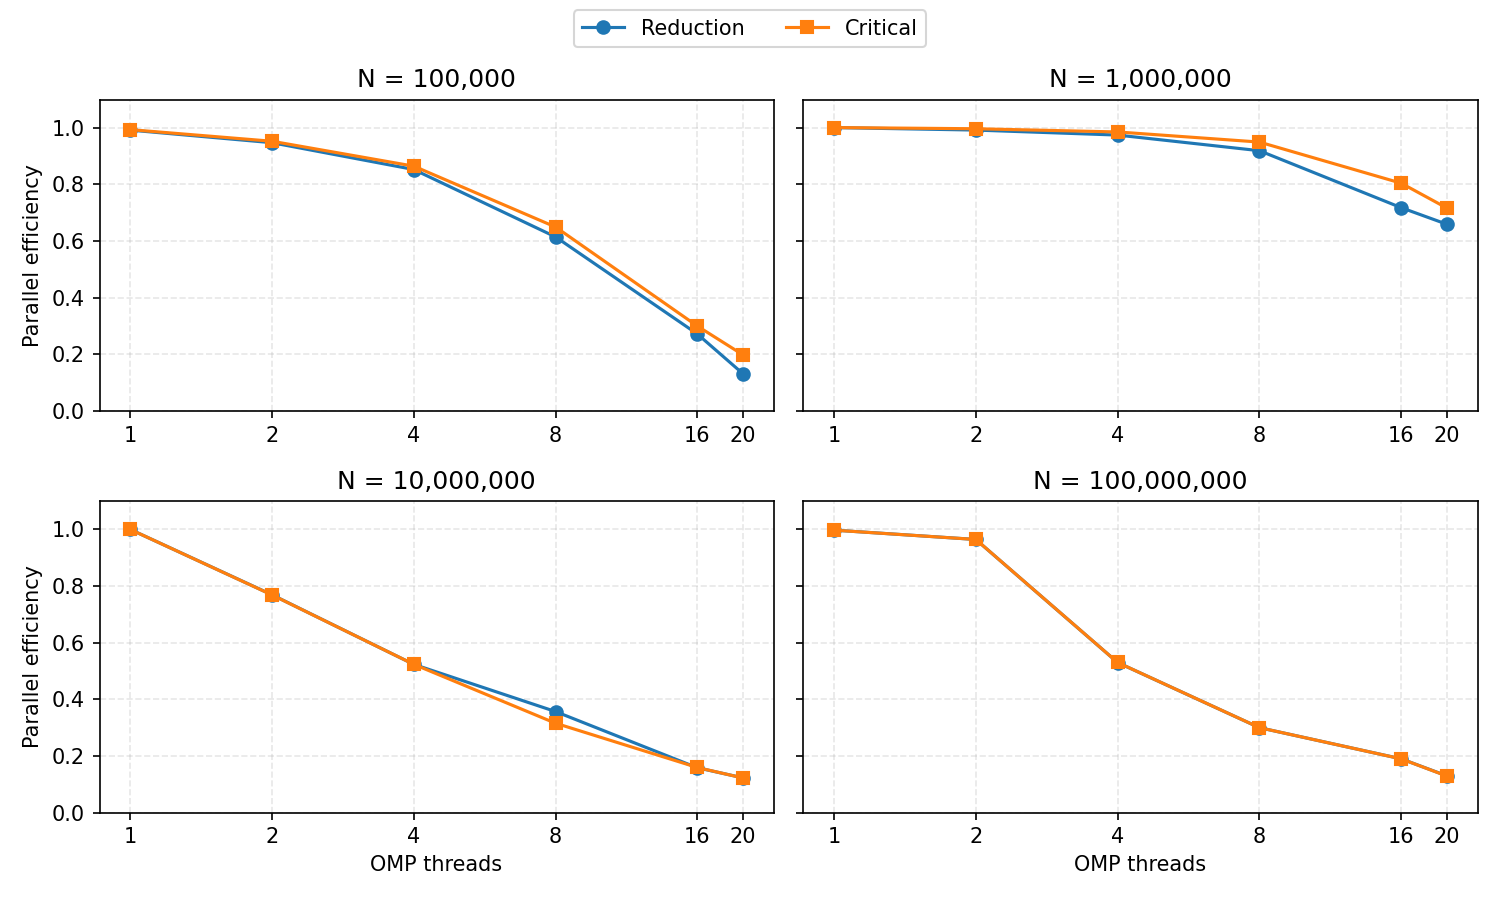
\includegraphics[width=0.75\linewidth]{../Skeleton_codes/dotProduct/plots/dotprod_efficiency.png}
    }{\fbox{Generate \texttt{dotprod\_efficiency.png} via \texttt{plot\_results.py}}}
    \caption{Parallel efficiency $E = T_1 / (p \cdot T_p)$ for the two OpenMP variants.}
    \label{fig:dotprod_eff}
\end{figure}

\subsection{Approximating $\pi$}

\section{The Mandelbrot set using OpenMP \punkte{20}}
\section{The Mandelbrot set using OpenMP \punkte{25}}

For this task, we developed two executables. The first, a serial program named \texttt{mandel\_seq.c}, iterates over every pixel in the complex plane, applying the iteration $z \leftarrow z^2 + c$ until either the magnitude of $z$ exceeds 2 or the maximum number of iterations, \texttt{MAX\_ITERS}, is reached. Each pixel's iteration count is stored in a temporary buffer, and a global counter \texttt{nTotalIterationsCount} accumulates the total iterations. The second executable, \texttt{mandel\_par.c}, retains the same computational kernel but parallelizes the pixel loop using \verb|#pragma omp parallel for|. It uses private variables for temporary computations and applies a \verb|reduction(+ : nTotalIterationsCount)| clause to safely sum the iteration counts across threads. To avoid race conditions during image writing, the PNG is generated only after the parallel region completes. A helper script, \texttt{run\_mandel.sh}, automates recompilation of both versions for four image resolutions ($1024^2$, $2048^2$, $4096^2$, and $8192^2$), runs the serial executable once per size, and then executes the OpenMP version with varying thread counts \texttt{OMP\_NUM\_THREADS} set to \{1, 2, 4, 8, 16, 20\}. Each run saves a log file in \texttt{Skeleton\_codes/mandel/logs/} and the corresponding PNG image in \texttt{Skeleton\_codes/mandel/png/}. \\

Example outputs for the two largest resolutions are shown in Figure~\ref{fig:mandel_images}.
\begin{figure}[H]
    \centering
    \begin{subfigure}{0.45\linewidth}
        
\includegraphics[width=\linewidth]{../Skeleton_codes/mandel/png/mandel_4096x4096_T20.png}
        \caption{4096×4096, 20 threads}
    \end{subfigure}
    \hfill
    \begin{subfigure}{0.45\linewidth}
        \includegraphics[width=\linewidth]{../Skeleton_codes/mandel/png/mandel_8192x8192_T20.png}
        \caption{8192×8192, 20 threads}
    \end{subfigure}
    \caption{Mandelbrot renderings generated by the OpenMP version.}
    \label{fig:mandel_images}
\end{figure}

\begin{figure}[H]
    \centering
    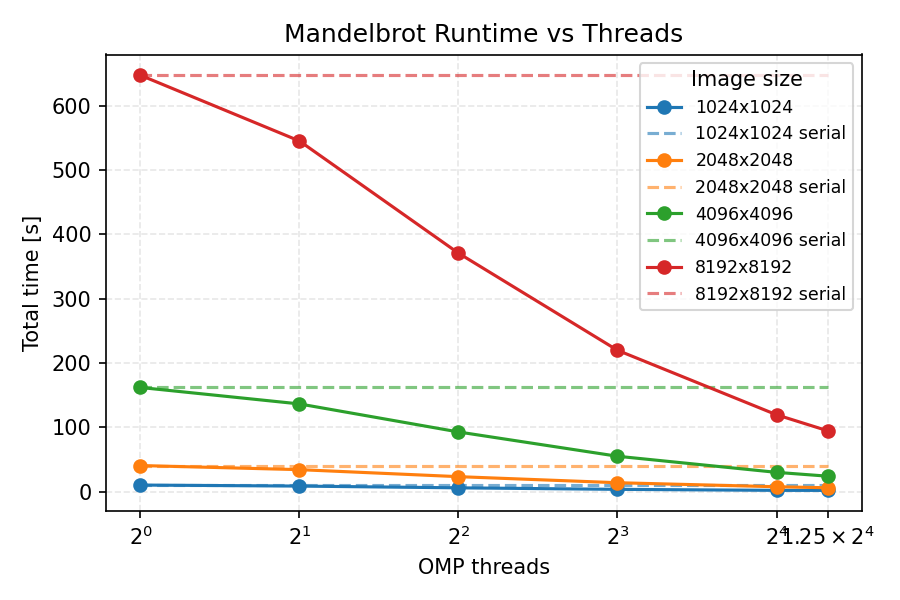
\includegraphics[width=0.75\linewidth]{../Skeleton_codes/mandel/plots/mandel_runtime_scaling.png}
    \caption{Total runtime versus thread count.}
    \label{fig:mandel_scaling}
\end{figure}

Table~\ref{tab:mandel_times} summarises the measured times (seconds) for the OpenMP binary; the serial baseline corresponds to the entry with one thread.
\begin{table}[H]
    \centering
    \begin{tabular}{c|rrrrrr}
        \hline
        Image size & Sequential & 2 threads & 4 threads & 8 threads & 16 threads & 20 threads \\
        \hline
        1024×1024 & 10.13 & 8.54 & 5.80 & 3.44 & 1.88 & 1.80 \\
        2048×2048 & 40.48 & 34.09 & 23.18 & 13.74 & 7.49 & 5.91 \\
        4096×4096 & 161.92 & 136.35 & 92.72 & 54.93 & 29.89 & 23.93 \\
        8192×8192 & 647.71 & 545.44 & 370.92 & 219.81 & 119.51 & 94.57 \\
        \hline
    \end{tabular}
    \caption{Total runtime for the OpenMP version; the iteration count remains constant across threads for each resolution.}
    \label{tab:mandel_times}
\end{table}

Looking at the curves in Figure~\ref{fig:mandel_scaling}, we see that using 20 threads gives us about a 5.6× speedup for the smallest image, and around 6.8× for larger ones. The dashed baselines line up with the measured points when using one thread, so it shows that the OpenMP setup doesn't add any extra overhead outside of the parallel region. For smaller images, the scaling levels off sooner since there’s less work per pixel, and the threads end up competing for memory bandwidth. But when we hit the $8192^2$ resolution, the workload for each thread is bigger, and the speedup stays pretty close to linear. In all cases, the iteration counter and the number of pixels logged match what we expected, which confirms that both the numerical kernel and the performance stats we were asked for are valid.

\section{Bug hunt \punkte{15}}
\section{Bug hunt \punkte{15}}


\section{Parallel histogram calculation using OpenMP \punkte{15}}
\section{Parallel histogram calculation using OpenMP \punkte{15}}


\section{Parallel loop dependencies with OpenMP \punkte{15}}
\section{Parallel loop dependencies with OpenMP \punkte{15}}

The sequential baseline in Listing~\ref{lst:recur_seq} computes the geometric recurrence
\mbox{$S_{n+1} = S_n\cdot\texttt{up}$} while storing every intermediate value in the array
\texttt{opt}.  This version is inherently schedule independent and serves as the reference for
both correctness and runtime.  The first parallel attempt (Listing~\ref{lst:recur_chunk}) keeps
the same arithmetic but splits the index range into contiguous chunks.  Each thread receives its
starting index, reconstructs the corresponding value through a single
\texttt{pow(up, start)} call, and then advances with repeated multiplications.  In OpenMP this is
implemented with \texttt{firstprivate(Sn)} so that every thread starts from the same scalar value;
no \texttt{lastprivate} is required because the final value is written in the shared 
\texttt{opt\_chunk} array.  The approach is fully schedule independent, because every thread owns
disjoint indices.

Listing~\ref{lst:recur_dyn} shows the second variant, where I experimented with a
\texttt{schedule(dynamic)} loop.  The idea was to keep using \texttt{firstprivate(Sn)} and
\texttt{lastprivate(Sn)} and to recompute the state only when a thread receives a non-contiguous
block.  The helper variables \texttt{Sn\_local} and \texttt{last\_i} were added precisely for
that purpose: whenever the assigned iteration is not the immediate successor of the previous one,
the code falls back to \texttt{Sn * pow(up, i)}.  Unfortunately this makes the loop depend on the
OpenMP scheduler.  With the default dynamic scheduler the runtime hands out extremely small
chunks, so the costly \texttt{pow} is executed almost every iteration.  As a consequence the
dynamic version violates the assignment requirement of being schedule independent and performs
worse than the serial baseline.

\lstinputlisting[
    language=C,
    numbers=left,
    caption={Sequential recurrence baseline},
    captionpos=b,
    label={lst:recur_seq},
    linerange={6-35},
    firstnumber=6
]{../Skeleton\_codes/loop-dependencies/recur_seq.c}

\lstinputlisting[
    language=C,
    numbers=left,
    caption={Chunk-based parallel recurrence},
    captionpos=b,
    label={lst:recur_chunk},
    linerange={21-37},
    firstnumber=21
]{../Skeleton\_codes/loop-dependencies/recur_omp.c}

\lstinputlisting[
    language=C,
    numbers=left,
    caption={Dynamic schedule with on-demand recomputation},
    captionpos=b,
    label={lst:recur_dyn},
    linerange={39-53},
    firstnumber=39
]{../Skeleton\_codes/loop-dependencies/recur_omp.c}

The scaling study (Figure~\ref{fig:recur_scaling}) confirms these observations.  The chunk-based
parallelisation reaches nearly linear speedup: the runtime drops from roughly $6.7\,$s on one
thread to $0.39\,$s on twenty threads.  The dynamic variant, on the other hand, keeps increasing
from $134\,$s (one thread) to $344\,$s (twenty threads), which is even slower than the serial
baseline at the far left of the plot.  The experiment therefore illustrates that the manual chunk
partitioning satisfies the “schedule independent’’ requirement of the assignment, whereas the
dynamic version is dominated by the repeated \texttt{pow} calls triggered by OpenMP’s fine-grained
work distribution.

\begin{figure}[H]
    \centering
    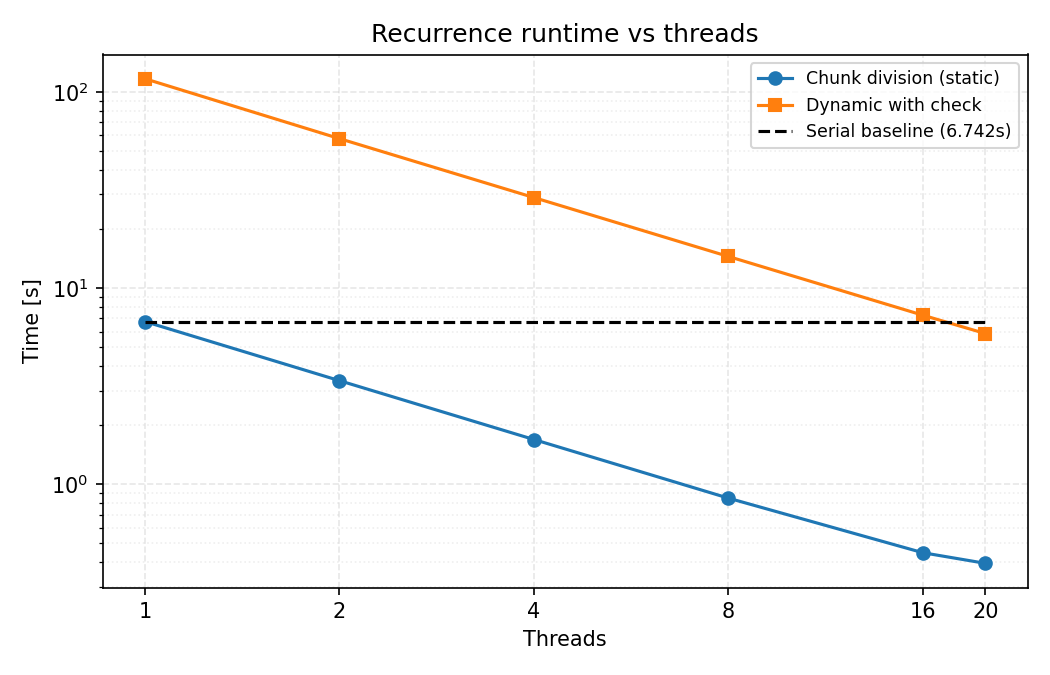
\includegraphics[width=0.75\linewidth]{../Skeleton\_codes/loop-dependencies/plots/recur_runtime_scaling.png}
    \caption{Runtime per thread count for the chunk and dynamic variants, compared with the serial baseline.}
    \label{fig:recur_scaling}
\end{figure}


\section{Quality of the Report \punkte{15}}



\end{document}
